\chapter{总体设计}
\section{软件描述}
系统包括考生用户子系统和ETS管理子系统两个部分。

考生子系统的主要功能是为考生用户提供以下服务:

1、注册成为系统的新用户

2、查询、更改自己的个人信息

3、查询考试时间、地点、考位信息

4、考试报名与取消报名

5、成绩查询

ETS管理子系统的主要功能是:

1、考试信息发布

2、题库维护

3、试题成型

4、试卷分发及测试

5、试卷批改

\section{处理流程}
\subsection{总体流程}

\subsection{系统基本流程}
\begin{figure}[ht]
\centering
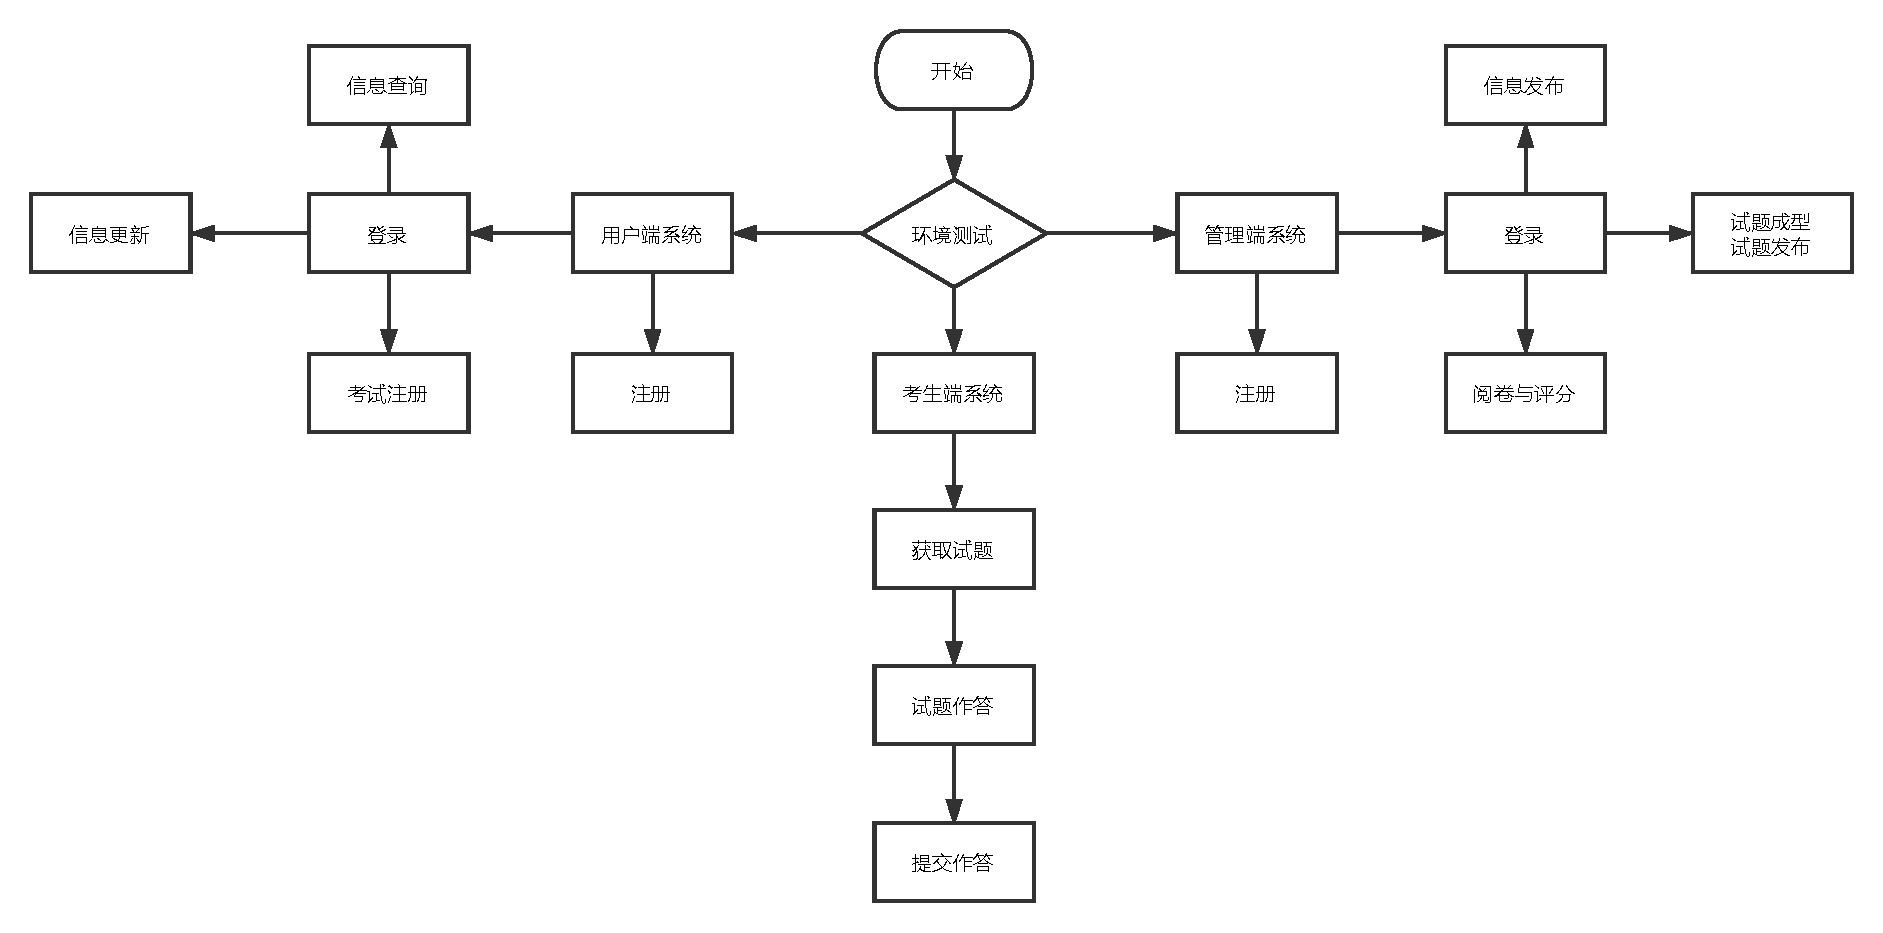
\includegraphics[width=10cm]{basic}
\caption{系统基本流程} \label{fig:figure1}
\end{figure}

用户先注册,向ETS系统提交其相关的个人信息,然后通过其用户名与密码登陆,进行后续操作。在登陆界面,用户可以查询个人信息、更新个人信息、查询并注册考试等。管理员同样需要进行受限的注册与登陆操作,然后可以进行考试信息发布、题目添加、试题成型、试卷分发、阅卷等操作。

\subsection{客户端基本流程}
\begin{figure}[ht]
\centering
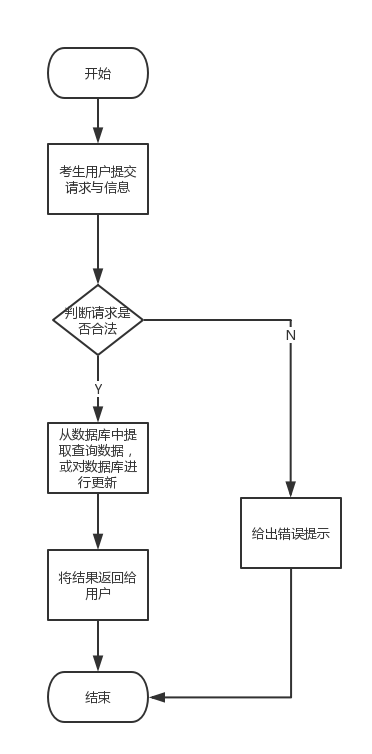
\includegraphics[width=10cm]{flowchart1.png}
\caption{考生用户子系统总体流程} \label{fig:figure2}
\end{figure}

上图是考生用户子系统总体流程图。系统接受用户的请求及附带的用户提供的信息,检测这些请求是否符合用户所具有的权限,以及检测用户所提交的信息是否符合要求。如果检测通过,则按照用户请求对数据库进行相应的增删改查等操作,并将操作结果返回给用户。否则,拒绝请求,并返回错误信息。

\subsection{服务器端基本流程}
\begin{figure}[ht]
\centering
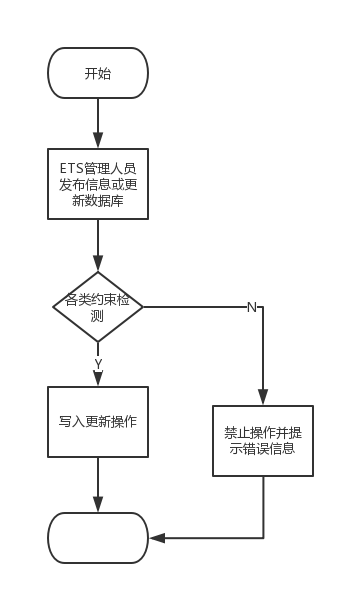
\includegraphics[width=10cm]{flowchart2.png}
\caption{ETS管理子系统总体流程} \label{fig:figure3}
\end{figure}

上图是ETS管理子系统总体流程图。系统接受用户提交的各类请求,验证用户身份及其所具有的权限,并进行完整性检查。如果检查通过,执行用户请求的操作。否则,拒绝操作并给出错误信息。

\subsection{注册功能具体流程}
\begin{figure}[ht]
\centering
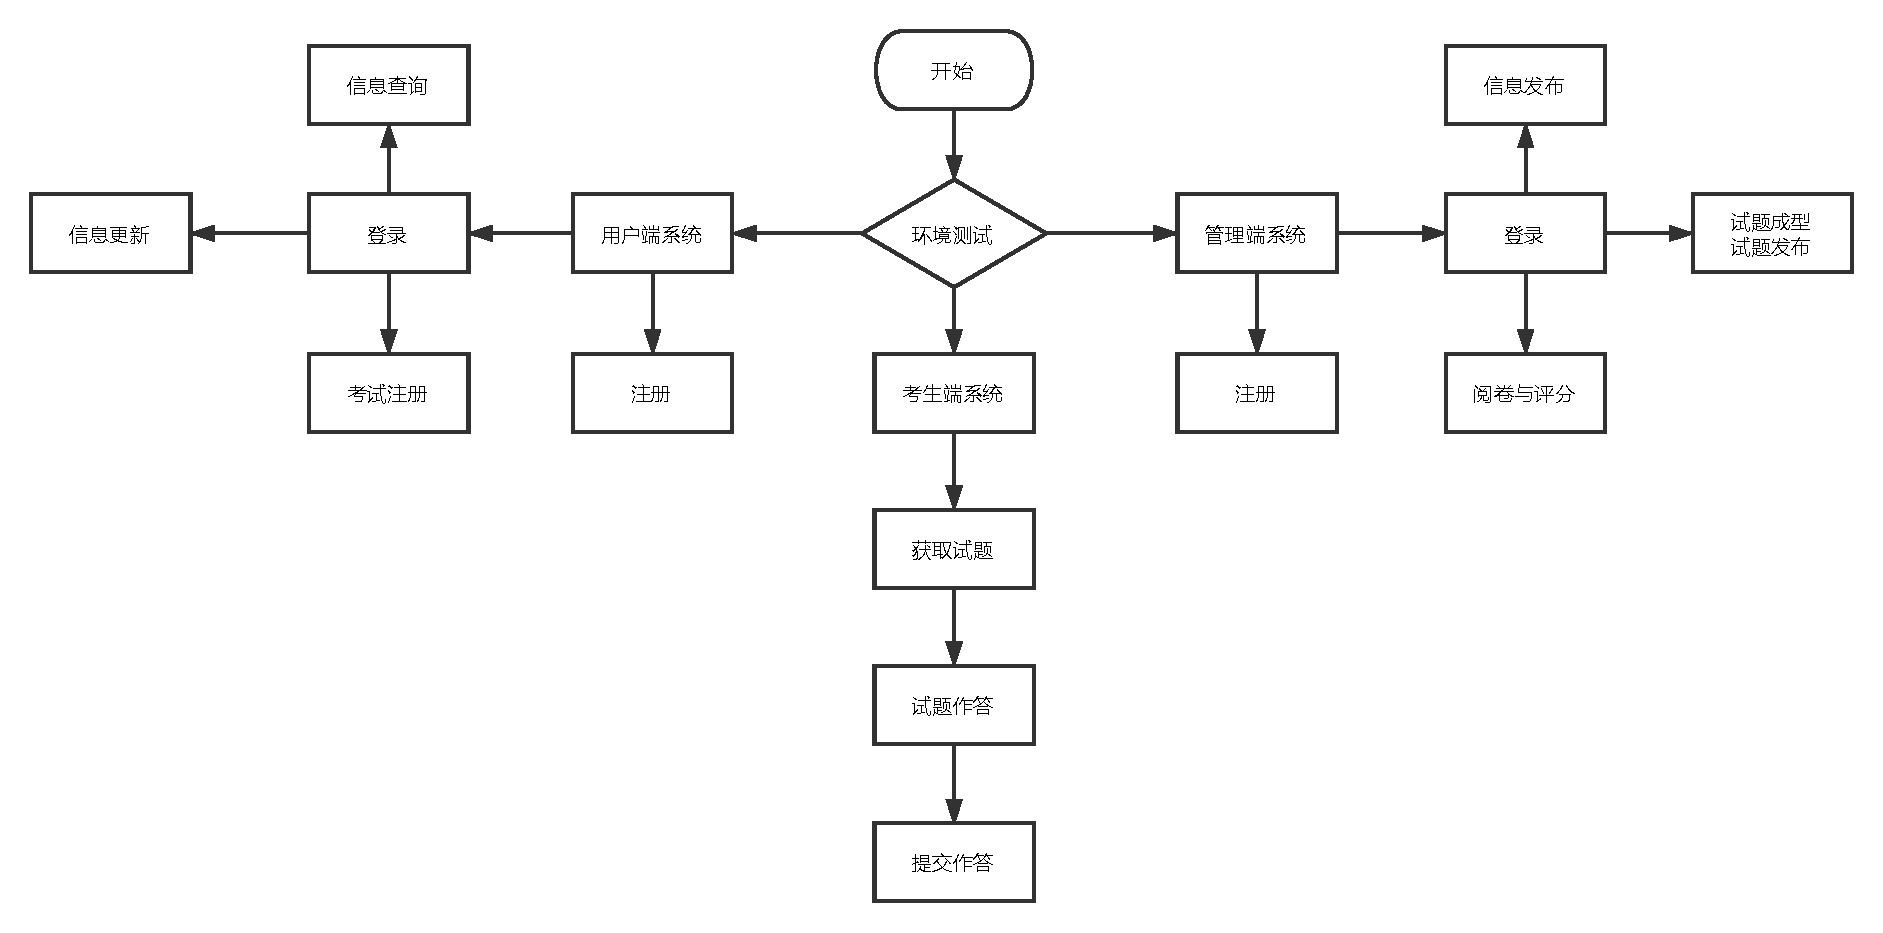
\includegraphics[width=10cm]{basic}
\caption{注册功能具体流程} \label{fig:figure4}
\end{figure}

用户向ETS系统发送注册请求后,ETS系统返回给用户具体的表单信息,用户根据提示,完善其用户名、密码、真实姓名、生日、身份证号、地址等信息,然后将表单提交给ETS系统,ETS系统根据用户提供的个人信息,检索其注册用户库,若发现重复,其生成新用户失败,返回提示信息,告知用户已存在相关账户,提示用户直接登录,否则,在数据库中录入用户个人信息,并告知用户已经注册成功,然后转入登录流程。

\subsection{登录功能具体流程}
\begin{figure}[ht]
\centering
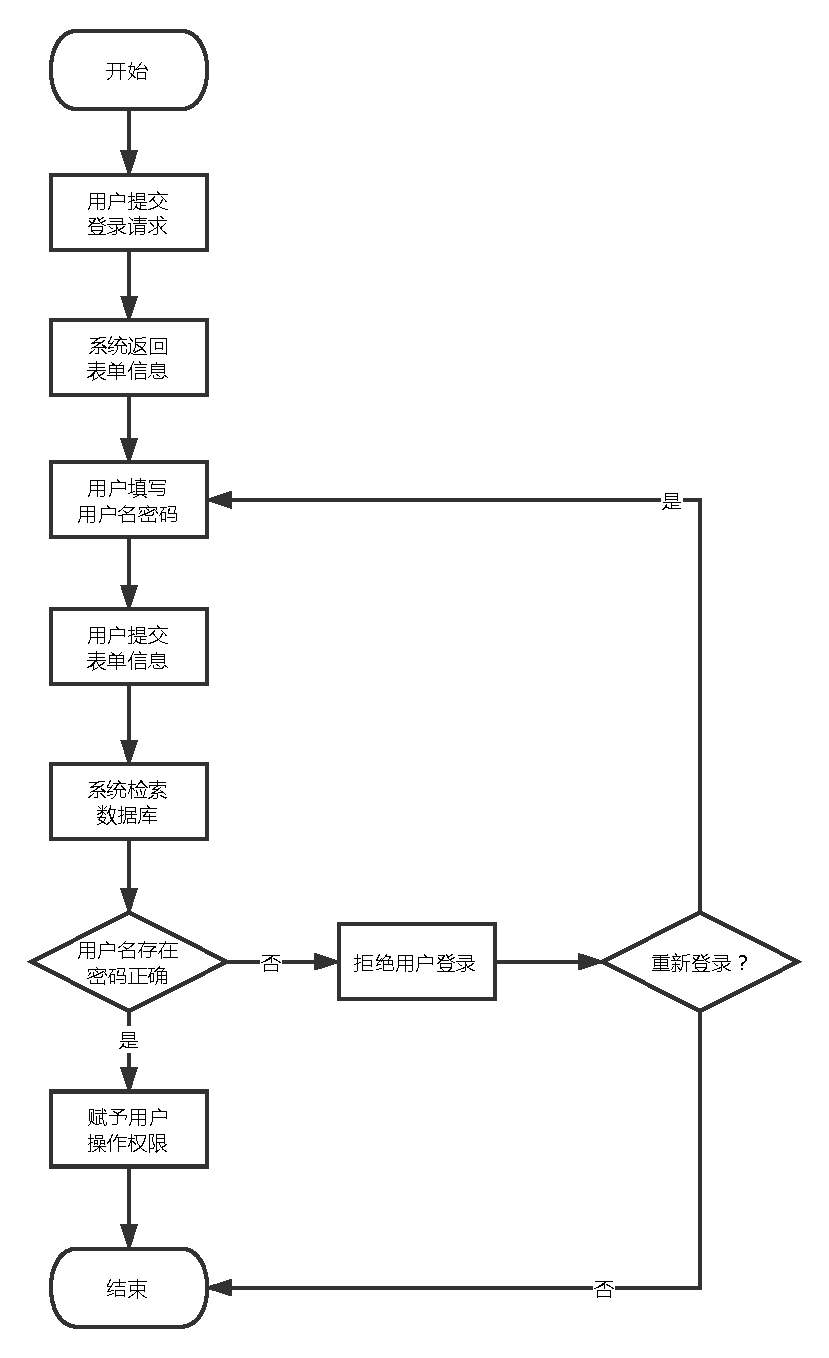
\includegraphics[width=10cm]{login}
\caption{登录功能具体流程} \label{fig:figure5}
\end{figure}

用户向ETS系统发送登录请求,ETS系统返回给用户具体的表单,要求用户输入其用户名和密码,用户输入完毕后,提交该表单信息,ETS系统根据表单信息检索数据库,若用户名存在,且密码与该用户名匹配,则返回给用户操作更多流程的权限,否则拒绝用户的进一步访问,要求用户重新提交用户名和密码。

\subsection{个人信息查询功能具体流程}
\begin{figure}[ht]
\centering
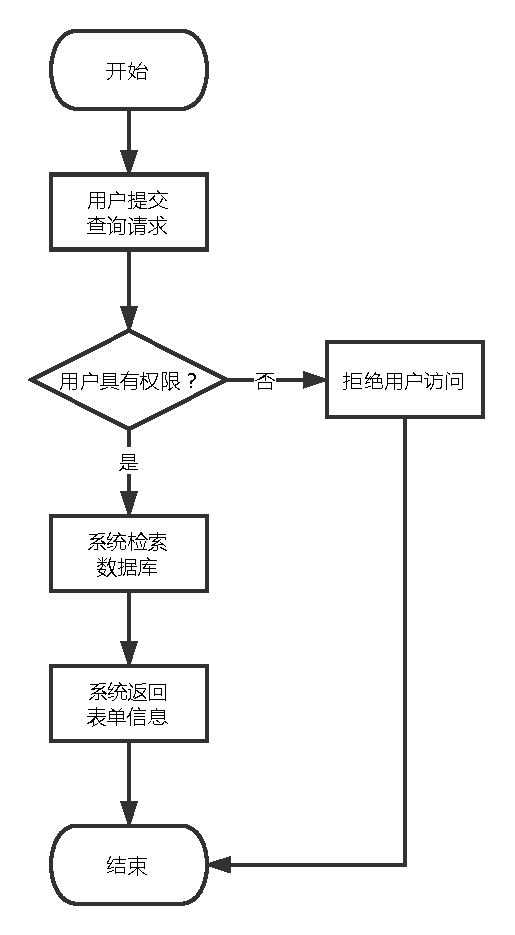
\includegraphics[width=10cm]{personal_info}
\caption{个人功能具体流程} \label{fig:figure6}
\end{figure}

用户向ETS系统发送查询请求,并指明查询的具体信息,ETS系统在接收到查询请求后,检查用户是否具有相应的查询权限,若有,则检索数据库系统,并返回相应的信息,否则返回提示信息,告知用户因权限不足访问被拒绝。

\subsection{考试信息发布功能具体流程}
\begin{figure}[ht]
\centering
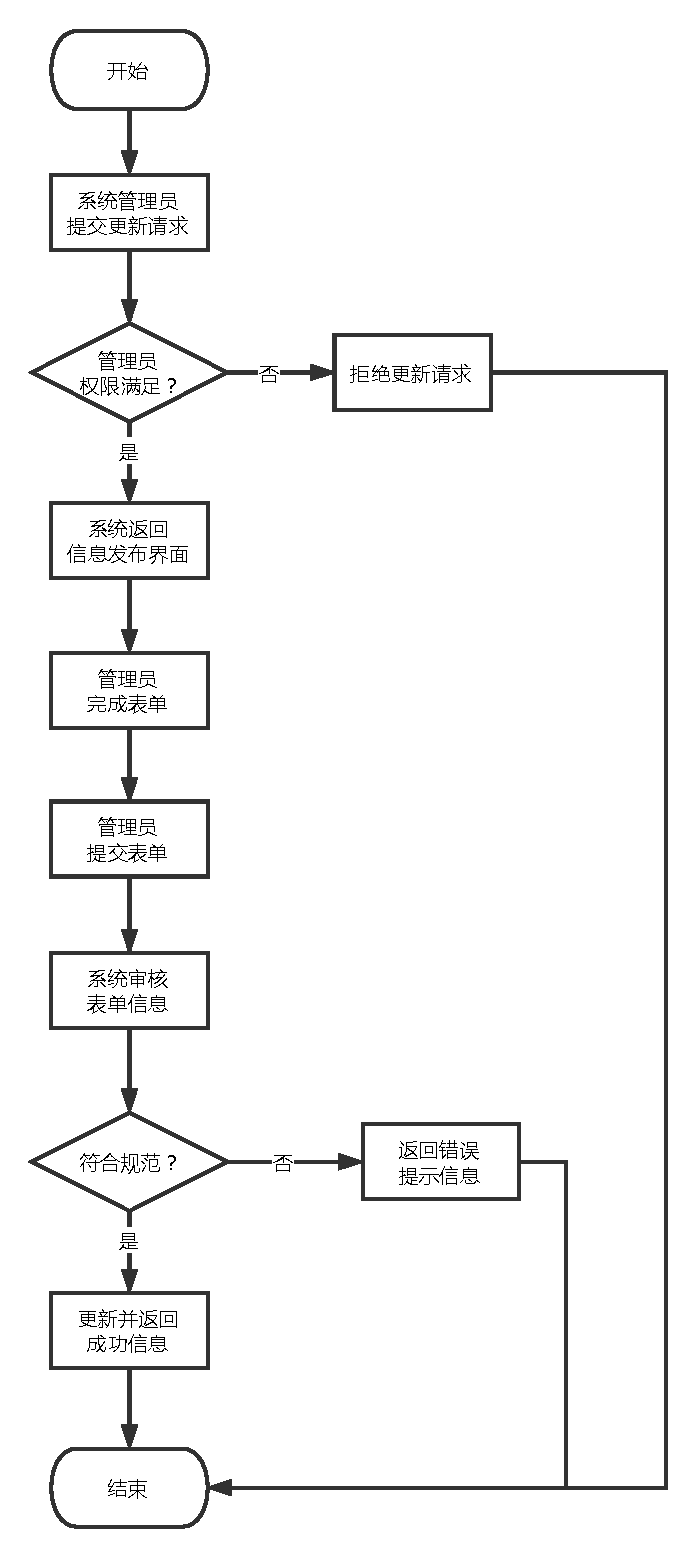
\includegraphics[width=10cm]{exam_info}
\caption{考试信息发布功能具体流程} \label{fig:figure7}
\end{figure}

ETS系统管理员向ETS系统发送考试信息更新请求,ETS系统在接收到请求后,检查ETS系统管理员的具体权限,若权限满足要求,则返回给ETS管理员发布考试信息的界面,否则拒绝其请求。ETS管理员在获取发布界面后,按照固定的程式,填写好考试相关信息,再提交ETS系统审核,ETS系统将根据已存在高级规则,对ETS管理员添加的考试信息进行查验,若满足相关发布规则,则更新其数据库,否则返回错误信息,要求ETS管理员对信息进行更正。

\subsection{试题成型功能具体流程}
\begin{figure}[ht]
\centering
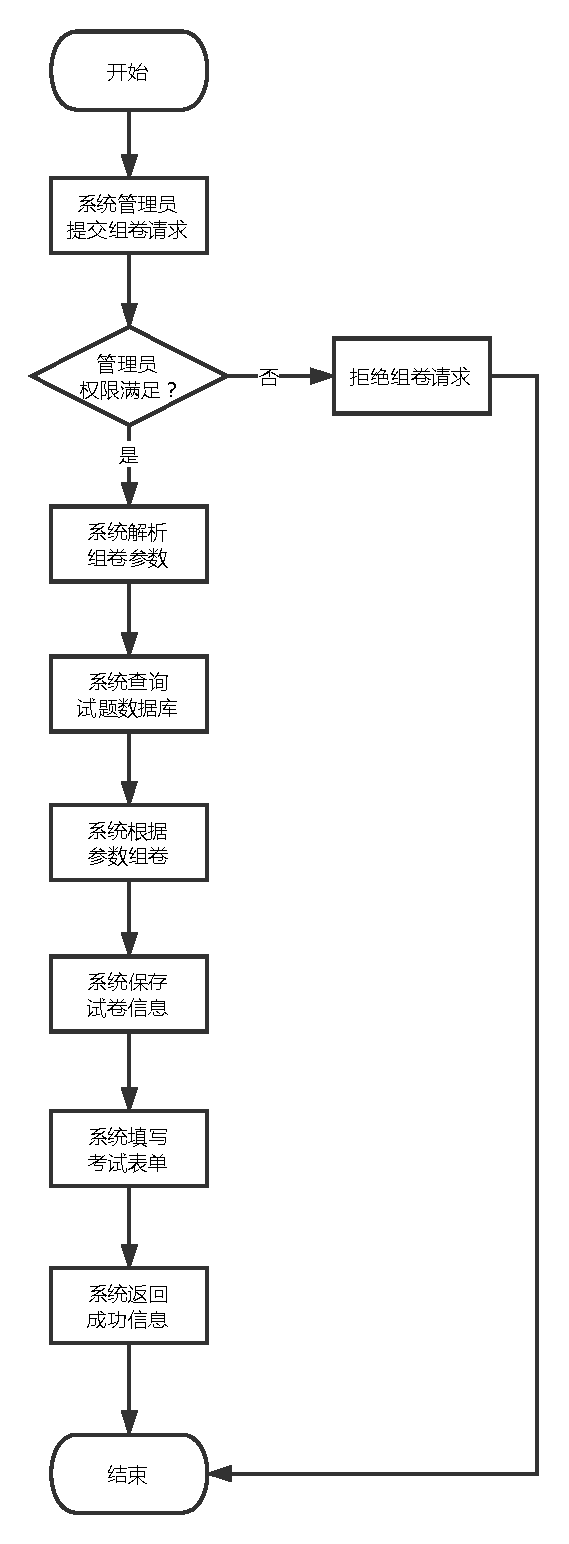
\includegraphics[width=8cm]{paper}
\caption{试题成型功能具体流程} \label{fig:figure8}
\end{figure}

ETS系统管理员向ETS系统发送组卷请求,并在该请求中,附带部分组卷参数,ETS系统在接收到请求后,解析组卷参数,然后查询数据库,按照参数所指定的组卷算法,生成一套试题,并将试题代号添加进与考试日期相关的表单中,然后返回成功信息,告知ETS管理员组卷成功。

\subsection{试卷分发与测试功能具体流程}
\begin{figure}[ht]
\centering
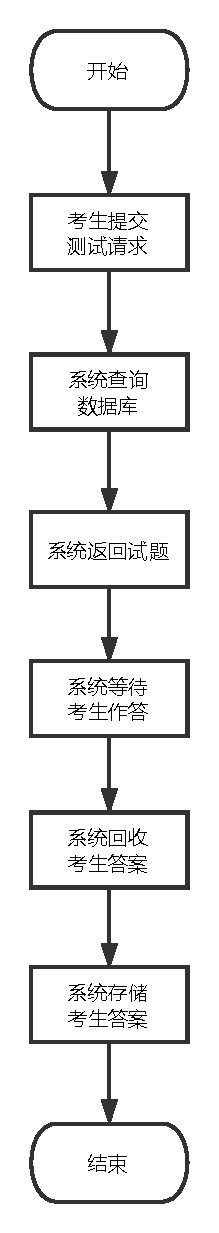
\includegraphics[width=4cm]{test}
\caption{试卷分发与测试功能具体流程} \label{fig:figure9}
\end{figure}

考生在考试界面上,向ETS系统发送测试请求,ETS以日期为关键字定位到具体考试,并检索该场考试的表单信息,提取试卷代号,然后在数据库中根据代号提取出完整试题,然后返回给考生测试的客户端界面,在考生测试完毕后,ETS系统接收到考生的提交请求,然后存储考生的作答信息,留待后续阅卷流程进行操作。

\subsection{试卷批改功能具体流程}
\begin{figure}[ht]
\centering
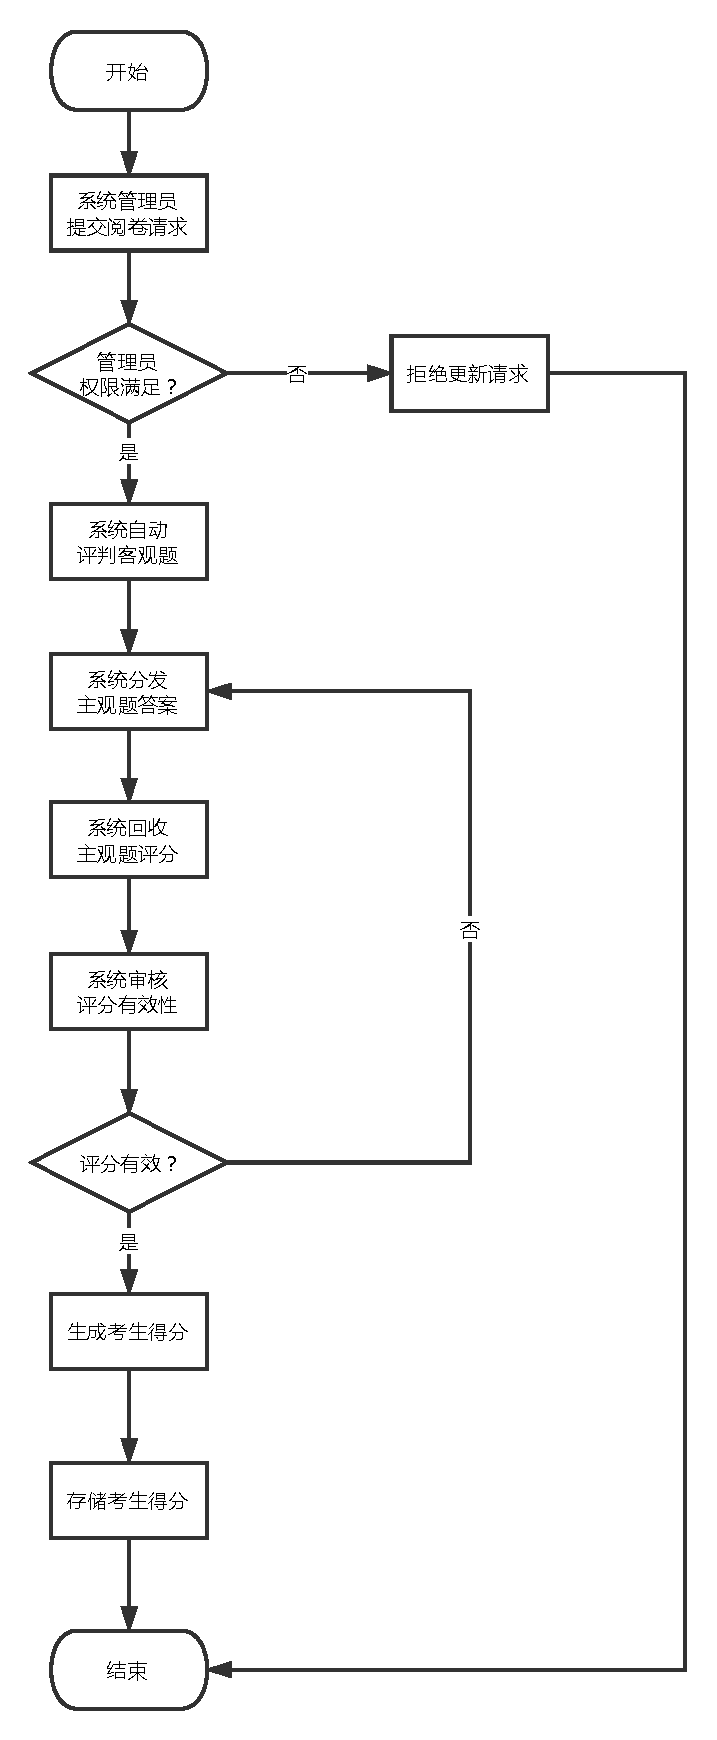
\includegraphics[width=10cm]{grading}
\caption{试卷批改功能具体流程} \label{fig:figure10}
\end{figure}

ETS管理员向ETS系统发送阅卷请求,ETS系统提取考生的客观题答题信息,与标准答案进行匹配,自动生成客观题部分的评分,之后,提取用户考生的主观题答题信息,根据ETS管理员所请求的参数,将考生答案提交给多位阅卷者,其中每位考生的每个答案,将同时提交给两位阅卷者,然后等待阅卷者返回分数信息。若阅卷者返回的同一考生的同一个作答的分数差异较大,则ETS系统将其提交给第三位权威阅卷者,否则则取其平均分作为考生该项目得分。


\section{功能结构设计}
\subsection{整体结构}
系统整体上分成两个模块,分别是考生用户子系统和ETS管理子系统。考生用户子系统处理考生用户提交的各类请求,ETS管理系统则提供更大权限,除了提供ETS方面提交的请求外,还可以对整个数据库有操作权限。

\subsection{用户端结构}
用户端特指考生用户子系统。它可以根据提供的服务划分不同的模块,包括用户注册模块、个人信息查询与更新模块、考试信息查询模块、考试报名模块、成绩查询模块等。它们之间没有耦合关系。

\subsection{服务器端结构}
服务器端特指ETS管理子系统。它也可以按照不同的服务划分不同的模块,包括考试信息发布、试题成型、试卷分发及测试、试卷批改各模块。其中,试卷批改模块依赖于试卷分发及测试模块,而试卷分发及测试模块依赖于试题成型模块。



\section{功能需求与程序代码的关系}
[此处指的是不同的需求分配到哪些模块去实现。可按不同的端拆分此表]
\begin{table}[htbp]
\centering
\caption{功能需求与程序代码的关系表} \label{tab:requirement-module}
\begin{tabular}{|c|c|c|}
    \hline
    · & 考生用户子系统 & ETS管理系统 \\
    \hline
    用户注册 & Y & · \\
    \hline
    个人信息查询与修改 & Y & · \\
    \hline
    考试信息查询 & Y & · \\
    \hline
    考试报名 & Y & · \\
    \hline
    成绩查询 & Y & · \\
    \hline
    考试信息发布 & · & Y \\
    \hline
    试题成型 & · & Y \\
    \hline
    试卷分发及测试 & · & Y \\
    \hline
    试卷批改 & · & Y \\
    \hline
\end{tabular}
\note{各项功能需求的实现与各个程序模块的分配关系}
\end{table}